\documentclass[twocolumn, 9pt]{article}
\usepackage{comment}
\usepackage{appendix}
\usepackage{cite}
\usepackage{fullpage} 
\usepackage[english]{babel}
\usepackage[utf8]{inputenc}
\usepackage{amsmath}
\usepackage{graphicx}
\usepackage[makeroom]{cancel}
\usepackage{multirow}
\usepackage[T1]{fontenc}
\usepackage[utf8]{inputenc}
\usepackage{authblk}
\usepackage{xcolor}
\usepackage{soul}
\usepackage{listings}
\usepackage{rotating}
\usepackage{pdflscape}
\usepackage[utf8]{inputenc}
\usepackage{listings}
\usepackage{natbib}
%\usepackage{hyperref}
%\usepackage{harvard}

\begin{document}
\title{Estimating Parameters of a Coupled ODE}

\author[1]{Eliot Heinrich}
\author[2]{Alexander Looi} 
\affil[1]{University of Vermont, Undergraduate}
\affil[2]{University of Vermont, Graduate}

\twocolumn
\maketitle
\section*{Abstract}
\indent{} blah blah blah blah blah blah blah blah blah blah blah blah blah blah blah blah blah blah blah blah blah blah blah blah blah blah blah blah blah blah blah blah blah blah blah blah blah blah blah blah blah blah blah blah blah blah blah blah blah blah blah blah blah blah blah blah blah blah blah blah blah blah blah blah blah blah blah blah blah blah blah blah blah blah blah blah blah blah blah blah blah blah blah blah blah blah blah blah blah blah blah blah blah blah blah blah blah blah blah blah blah blah blah blah blah blah blah blah blah blah blah blah blah blah blah blah blah blah blah blah blah blah blah blah blah blah blah blah blah blah blah blah blah blah. 

\section*{CCS Concepts}
\section*{Keywords}

\section{Introduction} 
\indent{} The goal of mathematical models is to be able to describe real properties and dynamics of the natural world. The original Lokta-Volterra Ordinary Differential Equations (ODE) aimed to describe the interactions of predator and prey through numerical values that describe specific properties. Many experiments and observational studies have provided evidence that this family of equations can describe the dynamics of real world predator prey interactions \cite{fussmann_crossing_2000, yoshida_rapid_2003, huffaker_experimental_1958, utida_cyclic_1957}. Additionally, many of these same studies were able to build ODE models that related simple behaviors and characteristics of predator and prey to the overall dynamics of the system. Take for example the growth rate of the prey, predator-prey models built using this parameter showed that a system two-species predator-prey system could transistion from stable coexistance, to stable limit cycles, and finally amplitudes with high extrema which resulted in extinction as prey growth rate was tune from low to high. \\
\indent{} It is known how variability in prey parameters (or bottom up forcing) can affect dynamics of the predator and thus the overall dynamics of a system \cite{smith_rosenzweig-macarthur_nodate, mccauley_physiological_1990, mccauley_growth_1990, mccauley_cyclic_1987, mccauley_large-amplitude_1999}. Less attention is given to the effect of tuning predator behavior (i.e. bottom up forcing). Some studies attempted to alter aspects of just predator efficacy in consuming prey. For example, Luckinbill \cite{luckinbill_coexistence_1973, luckinbill_effects_1974} was able to alter the encounter rate of predator and prey, both aquatic ciliates, by increasing viscosity of their medium. In this study salinity of the predator and prey media was used to tune the feeding rate of the predator, a marine rotifer. \\
\indent{} In this system, the predator has a much narrower optimal growth range compared to its algal prey \cite{snell_effect_1986, sarma_effect_nodate, miracle_salinity_nodate}. Additionally, experiments were conducted to document the dynamics between predator and prey. Then the below set of ODEs were used in an attempt to predict and accurately simulate the system.  \\
\begin{align}
    FcN = \frac{\beta_C*N}{(K_c+N)} \\
    FbC = \frac{\beta_R*C}{(K_r+C)} \\
    \frac{dN}{dt}=\delta*(80-N)-FcN*C \\
    \frac{dC}{dt}=FcN*C-(FbC*\frac{R}{e})-\delta*C \\
    \frac{dR}{dt}=FbC*R-(\delta+m)*R 
\end{align}

Here, $N$, $C$, and $R$ are the concentrations of nitrogen, chlorella (prey), and rotifers (predator) respectively. $\beta_C$ is the growth rate of the prey and $\beta_R$ is the growth rate of the predator. $K_c$ and $K_r$ are the half saturation constant of the prey and predator respectively \cite{fussmann_crossing_2000}. Lastly, $\delta$ is the flow through rate of the system (i.e. the dilution rate) and $m$ is the death rate of the predator.  

Models like this one need to accurately describe the data they aim to represent if researchers are to say that they understand the system that the data represent. However, initial simulations using known or experimentally derived parameters did not accurately portray the system predator-prey dynamics, which suggests our understanding of the system's parameters is flawed. Thus, to gain a better understanding of how parameters of this system of equations interact all fixed parameters were optimized given the original experimental data set using three techniques: 1) Single-Objective Differential Evolution (SODE), 2) Non-dominated Sorting Algorithm II (NSGAII), and 3) Spatial Pareto Evolutionary Algorithm 2 (SPEA2) \cite{deb_fast_2002, zitzler_spea2:_nodate}.

After optimizing multiple times and getting a suite of viable solutions (assuming that this problem exhibits non-uniqueness) we see if there are 1) multiple parameter sets that can describe a given data set given our current model of the system, and 2) how the parameter set may vary if the problem is non-unique. We can then see if our initial understanding of the system and how our choosen ODE was accurate.   

\section{Methods}

\indent{} The system of ODEs was optimized over the predator and prey abundance over time. Thus, to measure how well the simulations of a parameter set matched the data we used the mean squared error (MSE) for both predator and prey. However, this poses a slight problem becuase this means we have two values or objectives in a fitness function. Thus, three techniques with two different types of objectives were used to optimize the system of ODEs. The SODE technique is a single-objective, meaning there was only one value that needed to be optimized. NSGAII and SPEA2 are multi-objective (MO) techniques, meaning these algorithms optimized over two values. This culminated in this study using two different fitness functions. 

\subsection{Fitness Functions:}

In this study the distance between the simulated data produced from a set of estimated parameters and the actual (experimental) data was minized. There are two species (the predator and prey), thus we need fitness functions that can appropriately capture the error between the simulations and the data of both, and still guide our algorithms to the best solution. Additionally, we only care about the absolute deviation from data and want to severely penalize large deviations from the data; this is why we used MSE.

In the MO case we gave the algorithms the MSEs of the predator and the prey. Because NSGAII and SPEA2 are MO we simply passed both the MSE of predator and prey to these algorithms.  

However, for the SO fitness function we added the errors of the predator and the prey. However, there is the potential for the MSE of the prey to dominate the fitness function because the numerical units of the prey are greater than the predator (millions of individuals vs several). Thus, to avoid this error imbalance when combing the predator and prey MSE we used the Root Mean Squared Error (RMSE).
\begin{align}
    MSE=\frac{1}{n}\sum_{i=1}^{n} (Y_i - Y)^2 \\
    RMSE=\frac{\sqrt{\frac{1}{n}\sum_{i=1}^{n} (Y_i - Y)^2}}{mean(Y)}
\end{align}

By square rooting the MSE value, we obtain the original units of the predator and prey error. Then by dividing by the mean of the data, we can normalize the absolute value of the MSE. Then the final predator and prey RMSE values are simply added together. In this final form the prey will not dominate the fitness function unless simulations significantly deviate from the data.  

\subsection{Experiments:}

As a control we compared the results of the GAs to two gradient descent algorithms: Nelder-Mead (NM) and the Limited Memory Broyden–Fletcher–Goldfarb–Shanno (BFGS). We ran the gradient descent algorithms at 30 different random seeds to get a variety of solutions. The SOBE were run at the same 30 random seeds with a population of 1000 individuals and were allowed to run until the function self terminated. The best inidividual at the end of these thirty runs was taken as data to explore how parameters vary among the best solutions.

The MO algorithms were run for 100,000 generations with a population of 1,000 individuals. The best 31 individuals (15 individuals on either side of the best solution) of the final Pareto set of solutions were taken as best solutions and these parameter sets were used as the data to explore how parameters vary among the best solutions. Lastly, for all algorithms used, the range of acceptable parameter values were bounded so that parameter values estimated by our algorithms remained plausible, or at least within the range observed in our studies \ref{table:Bounds}. 
% table about the parameter bounds and the initial values used that were derived from experiments. 

\section{Results}

Figure \ref{fig:SigmaParameterSols} shows the parameter estimates for each algorithm. The two gradient descent methods (L-BFGS-B and Nelder-Mead) always found the same set of parameter values. As expected the two gradient descent methods never found the same set of parameter values across the different levels of noise despite the data being generated from a common parameter set. Additionally, all algorithms produced populations of unique parameters across all the levels of noise (Kruskal-Wallis Test at an $\alpha$ value of 0.05).

% the bimodal distributions suggest that there are two or more parameter sets that are "strong" candidates as good solutions given the data set. Don't really see this in the generate data. Hard to tell if this is because of noise in the experimental data or something else. The fact that there is noise in the generated data suggests that the non-uniqueness is not because of noise in the experimental data and could be a trait of the predator and prey interaction. 
\section{Discussion}

\section{Conclusions}

% References here
{\footnotesize
\bibliographystyle{unsrt}
\bibliography{ECProjectRefs}
}
\onecolumn
% figures and tables go here
% representative runs showing estimated data, and the real/generated Data
% table 1 Parameter Bounds and Sources
\begin{table}[ht]
	\caption{Parameter bounds used in all optimization techniques discussed in this paper. Included are the sources for the parameter bounds and initial estimates at the four different experimental salinities (these are unpublished data based on experiments).}
    \hrule
    \small
    \begin{tabular}{l l}
    	\label{table:Bounds} % table for the Bounds
        	\begin{tabular}{c c c}
        	Parameter & Bound & Source \\
        	\cline{1-3}
        	$\beta_C$ & 1.0 25.0 & \cite{fussmann_crossing_2000, wen_biological_2005}  \\
            $K_c$ & 1.0 - 10.0 & \cite{laliberte_regulation_1989, ahmad_nitrogen_1984} \\
            $e$ & 0.01 - 0.5 & \cite{malekzadeh_viayeh_population_2010, snell_effect_1986}\\
            $m$ & 0.0 - 1.0 & Unpublished Data\\
            $\beta_R$ & 1.0 - 25.0 & \cite{doohan_energy_1973, peredo-alvarez_combined_nodate}\\
            $K_r$ & 1.0 - 50.0 & \cite{cheng_effects_2011, lowe_evidence_2005, yufera_factors_nodate}\\
        	\cline{1-3}
    	\end{tabular}
    	&
    	\label{table:Bounds} % table for the Bounds
        	\begin{tabular}{c c c c c}
        	Parameter & 3$gL^{-1}$ & 16$gL^{-1}$ & 35$gL^{-1}$& 45$gL^{-1}$ \\
        	\cline{1-5}
        	$\beta_C$ & 3.3 & 3.3 & 3.3 & 3.3 \\
            $K_c$ & 4.3 & 4.3 & 4.3 & 4.3 \\
            $e$ & 0.25 & 0.25 & 0.25 & 0.25 \\
            $m$ & 0.3 & 0.56 & 0.2 & 0.3 \\
            $\beta_R$ & 1.00 & 2.16 & 2.4 & 1.00 \\
            $K_r$ & 15 & 15 & 15 & 15 \\
        	\cline{1-5}
    	\end{tabular}
    \end{tabular}
    \hrule
\end{table}

% Figure showing parameter values estimated using the Generated Data
\begin{figure}[ht]
    \centering
    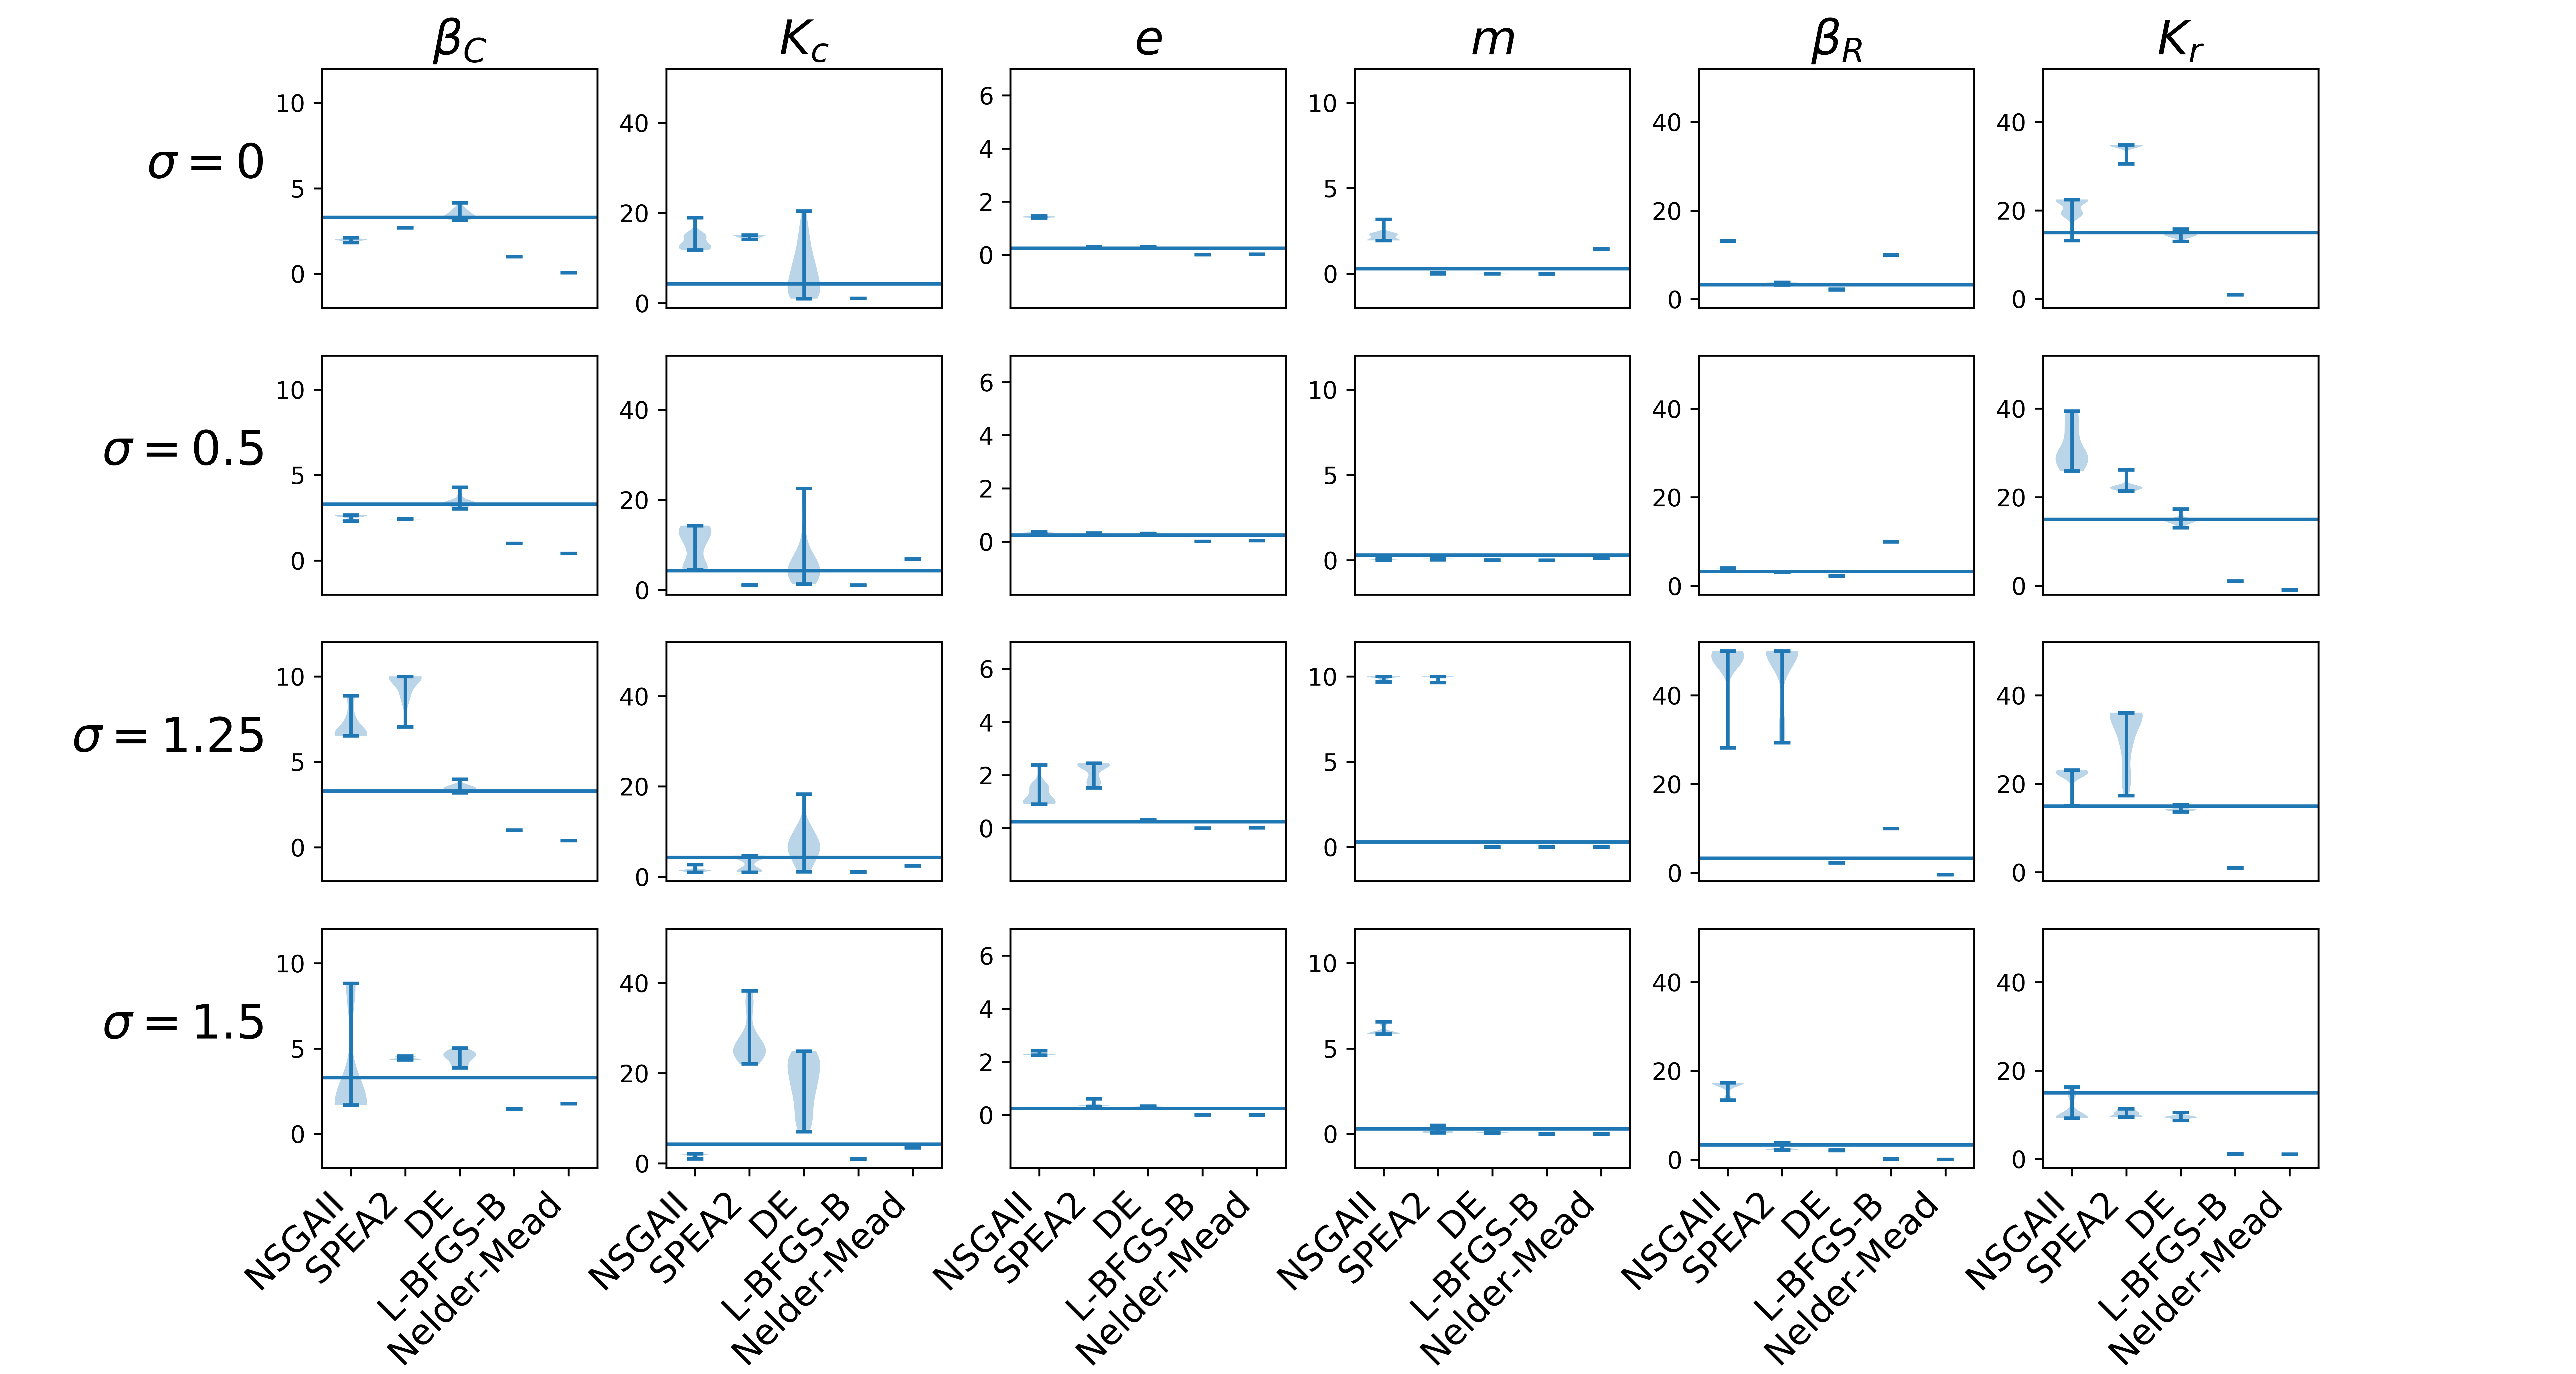
\includegraphics[width=\textwidth]{sigmaParameterFig.png}
    \caption{Parameter value distribution estimated by each algorithm, at different sigma values (i.e. different amounts of noise). Horizontal lines indicate the position the actual parameter value used to generate the original data set.}
    \label{fig:SigmaParameterSols}
\end{figure}

\begin{figure}[ht]
    \centering
    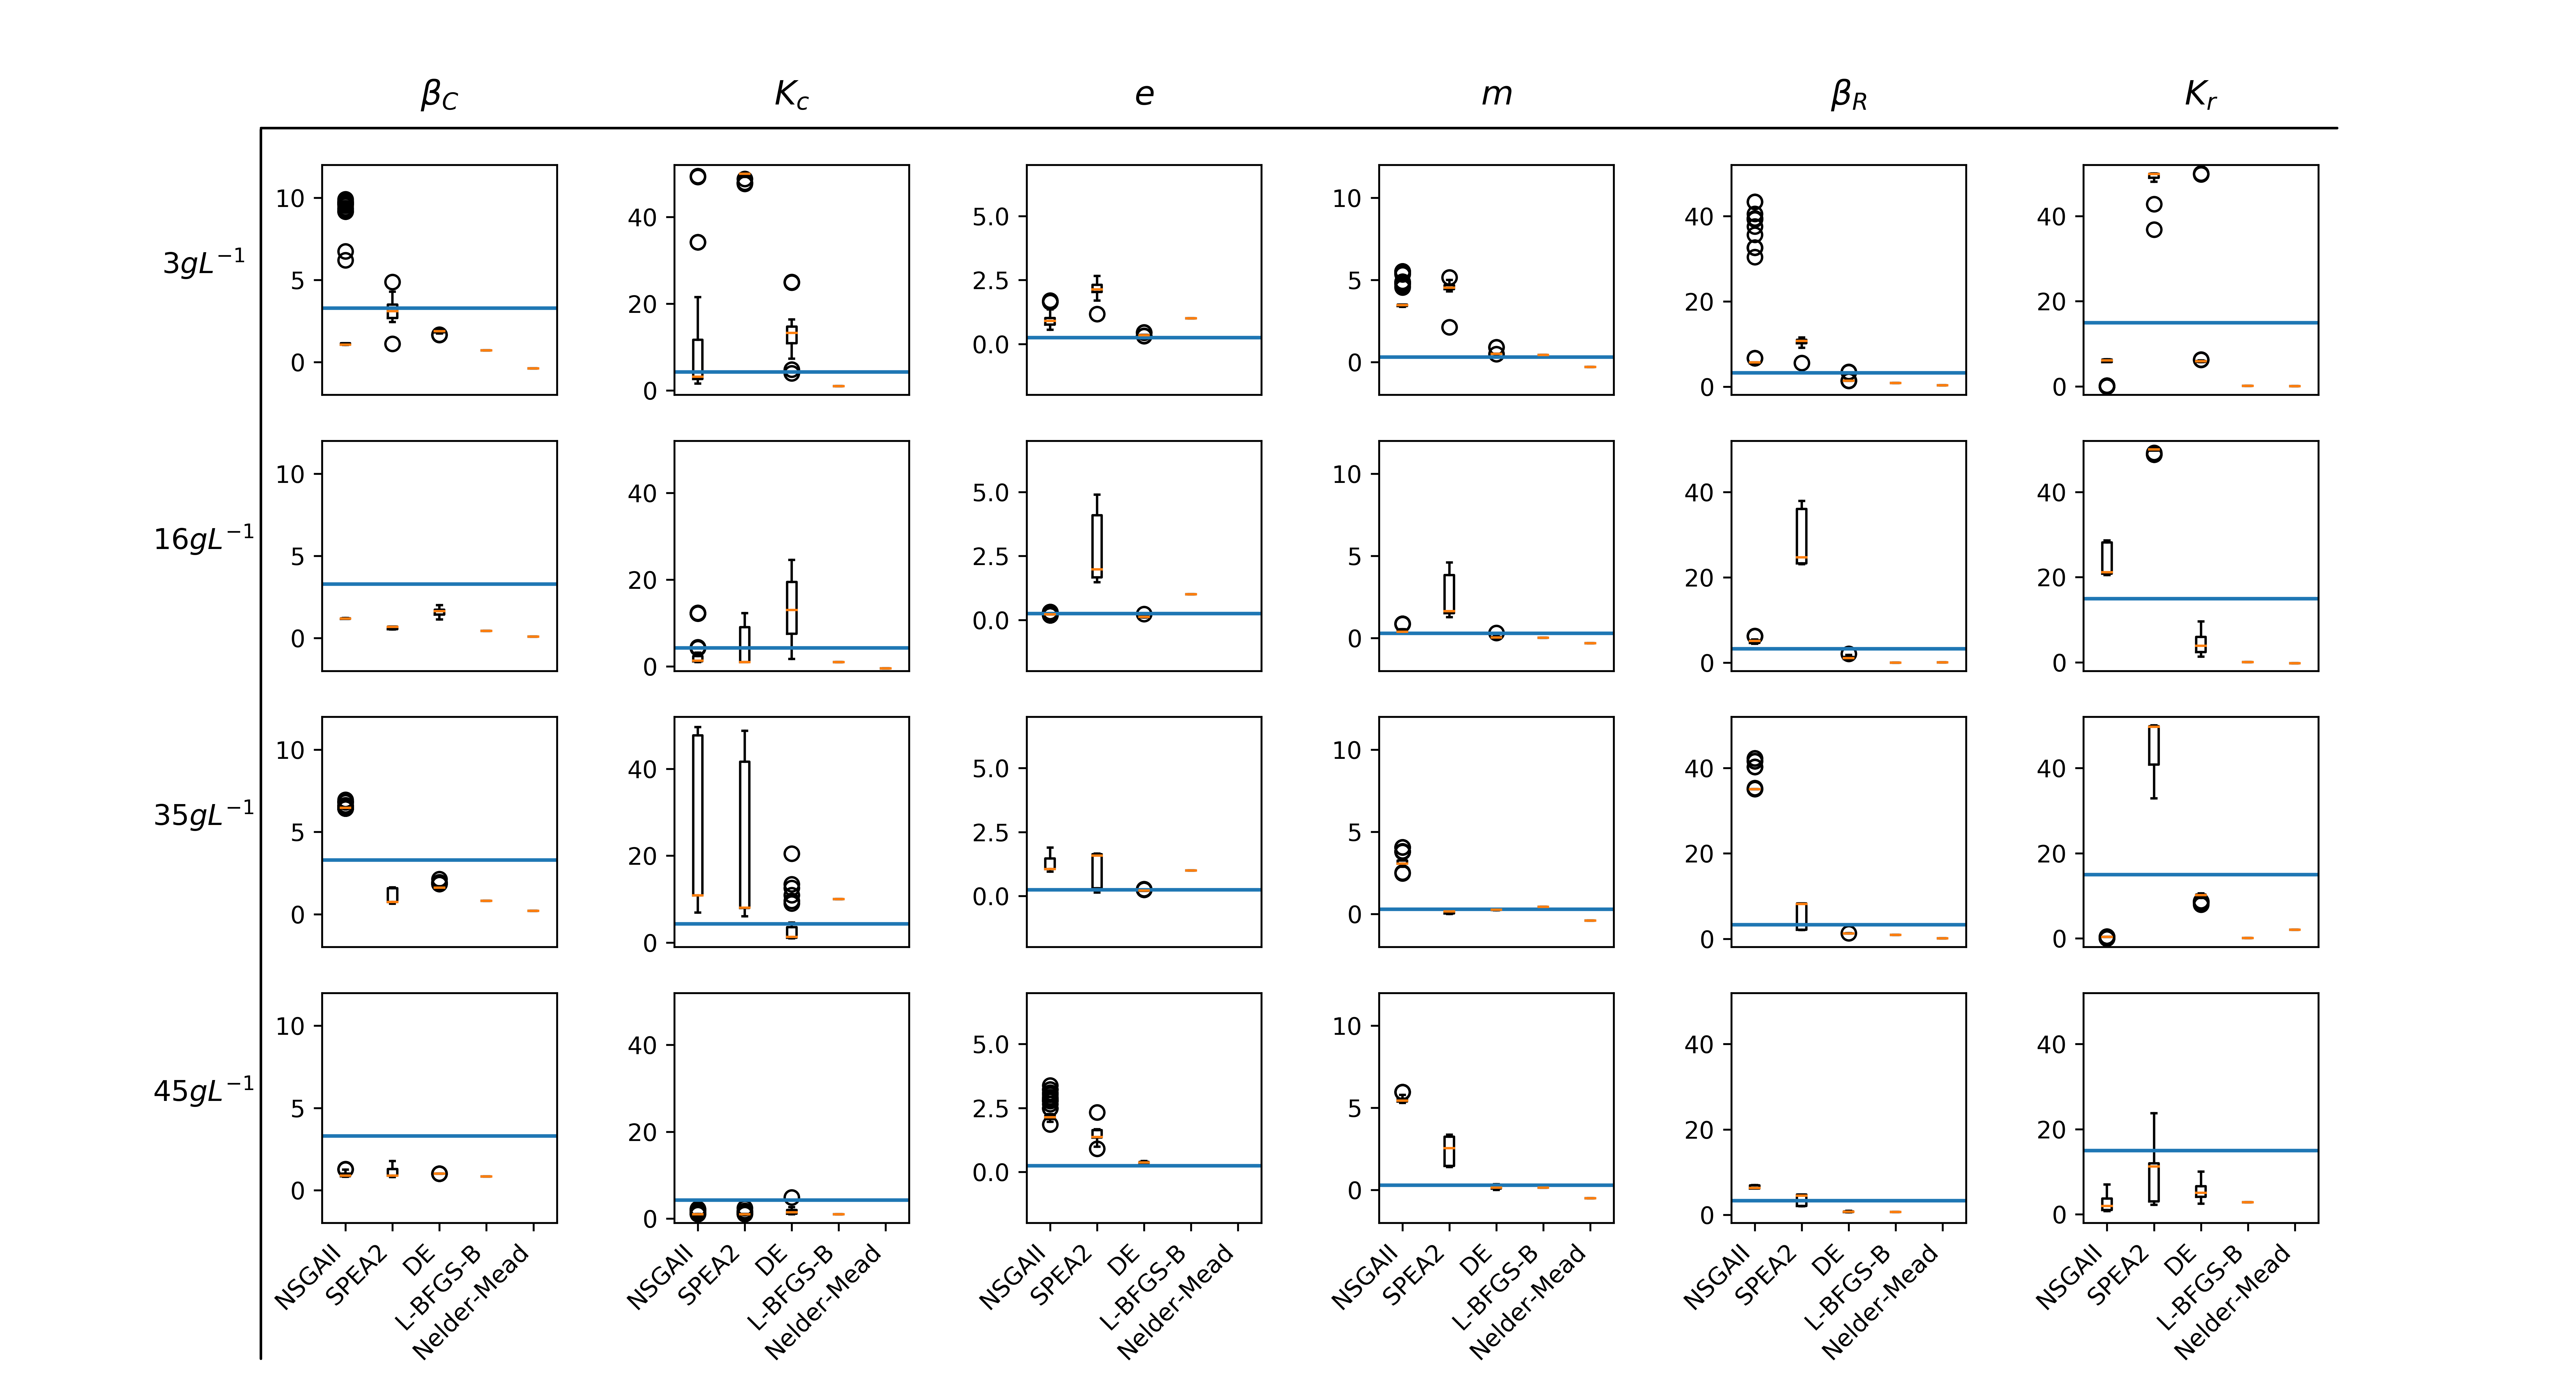
\includegraphics[width=\textwidth]{ParameterFig.png}
    \caption{Parameter value distribution estimated by each algorithm for different salinity levels in the experimental data set. Horizontal lines indicate the position of initial estimates of the parameter values provided by in lab experiments.}
    \label{fig:ParameterSols}
\end{figure}

\newpage
\section*{Appendix}
\indent{} Below are figures showing the that all algorithms used to solve the problem converged to some sort of minimum. Figure ~\ref{fig:DESOConvergence} shows the convergence of the SODE algorithm. The algorithm converged for all real data problems, however, there is a wide range of values even for the RMSE for all the random seeds used. This indicates that there may have been many local minimums that the algorithm found.
% Figure showing Convergence of data
\begin{figure}[ht]
    \centering
    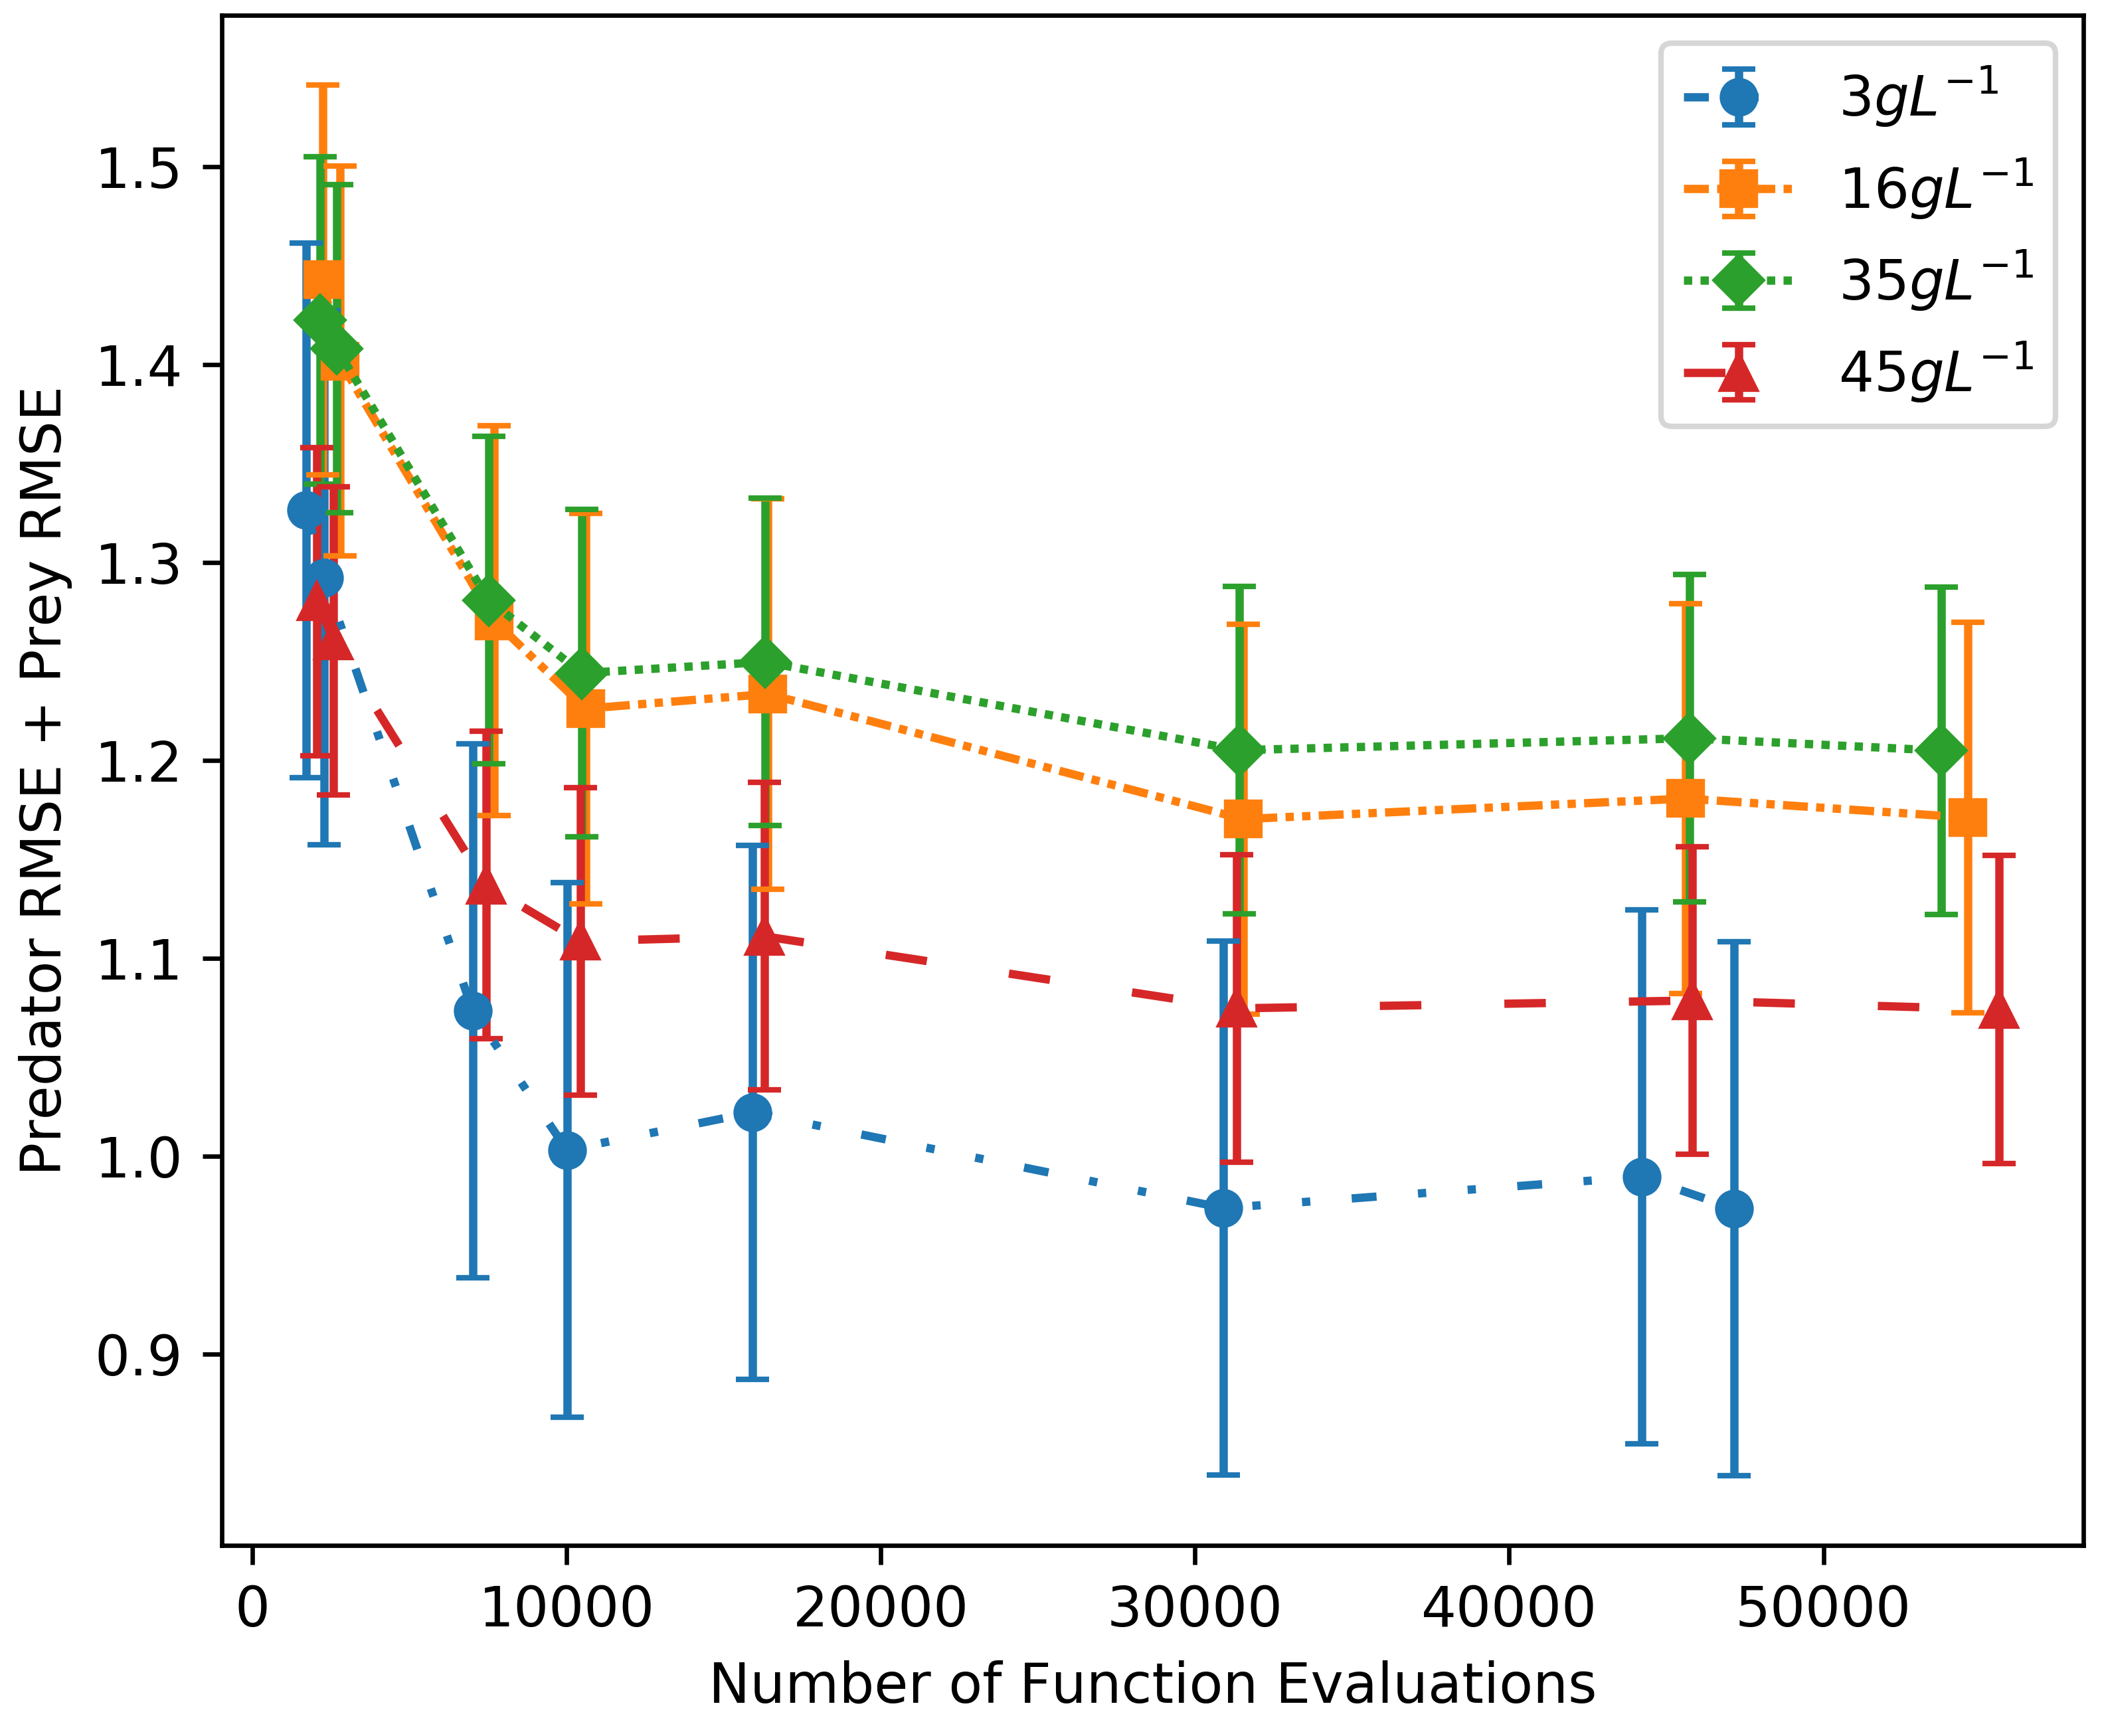
\includegraphics[width=0.60\textwidth]{DESOConvergence.png}
    \caption{Convergence of the SODE algorithm for each of the four data experimental data sets. Each point is the mean objective function value across all random seeds. Bars represent the standard deviation.}
    \label{fig:DESOConvergence}
\end{figure}

\begin{figure}[ht]
    \centering
    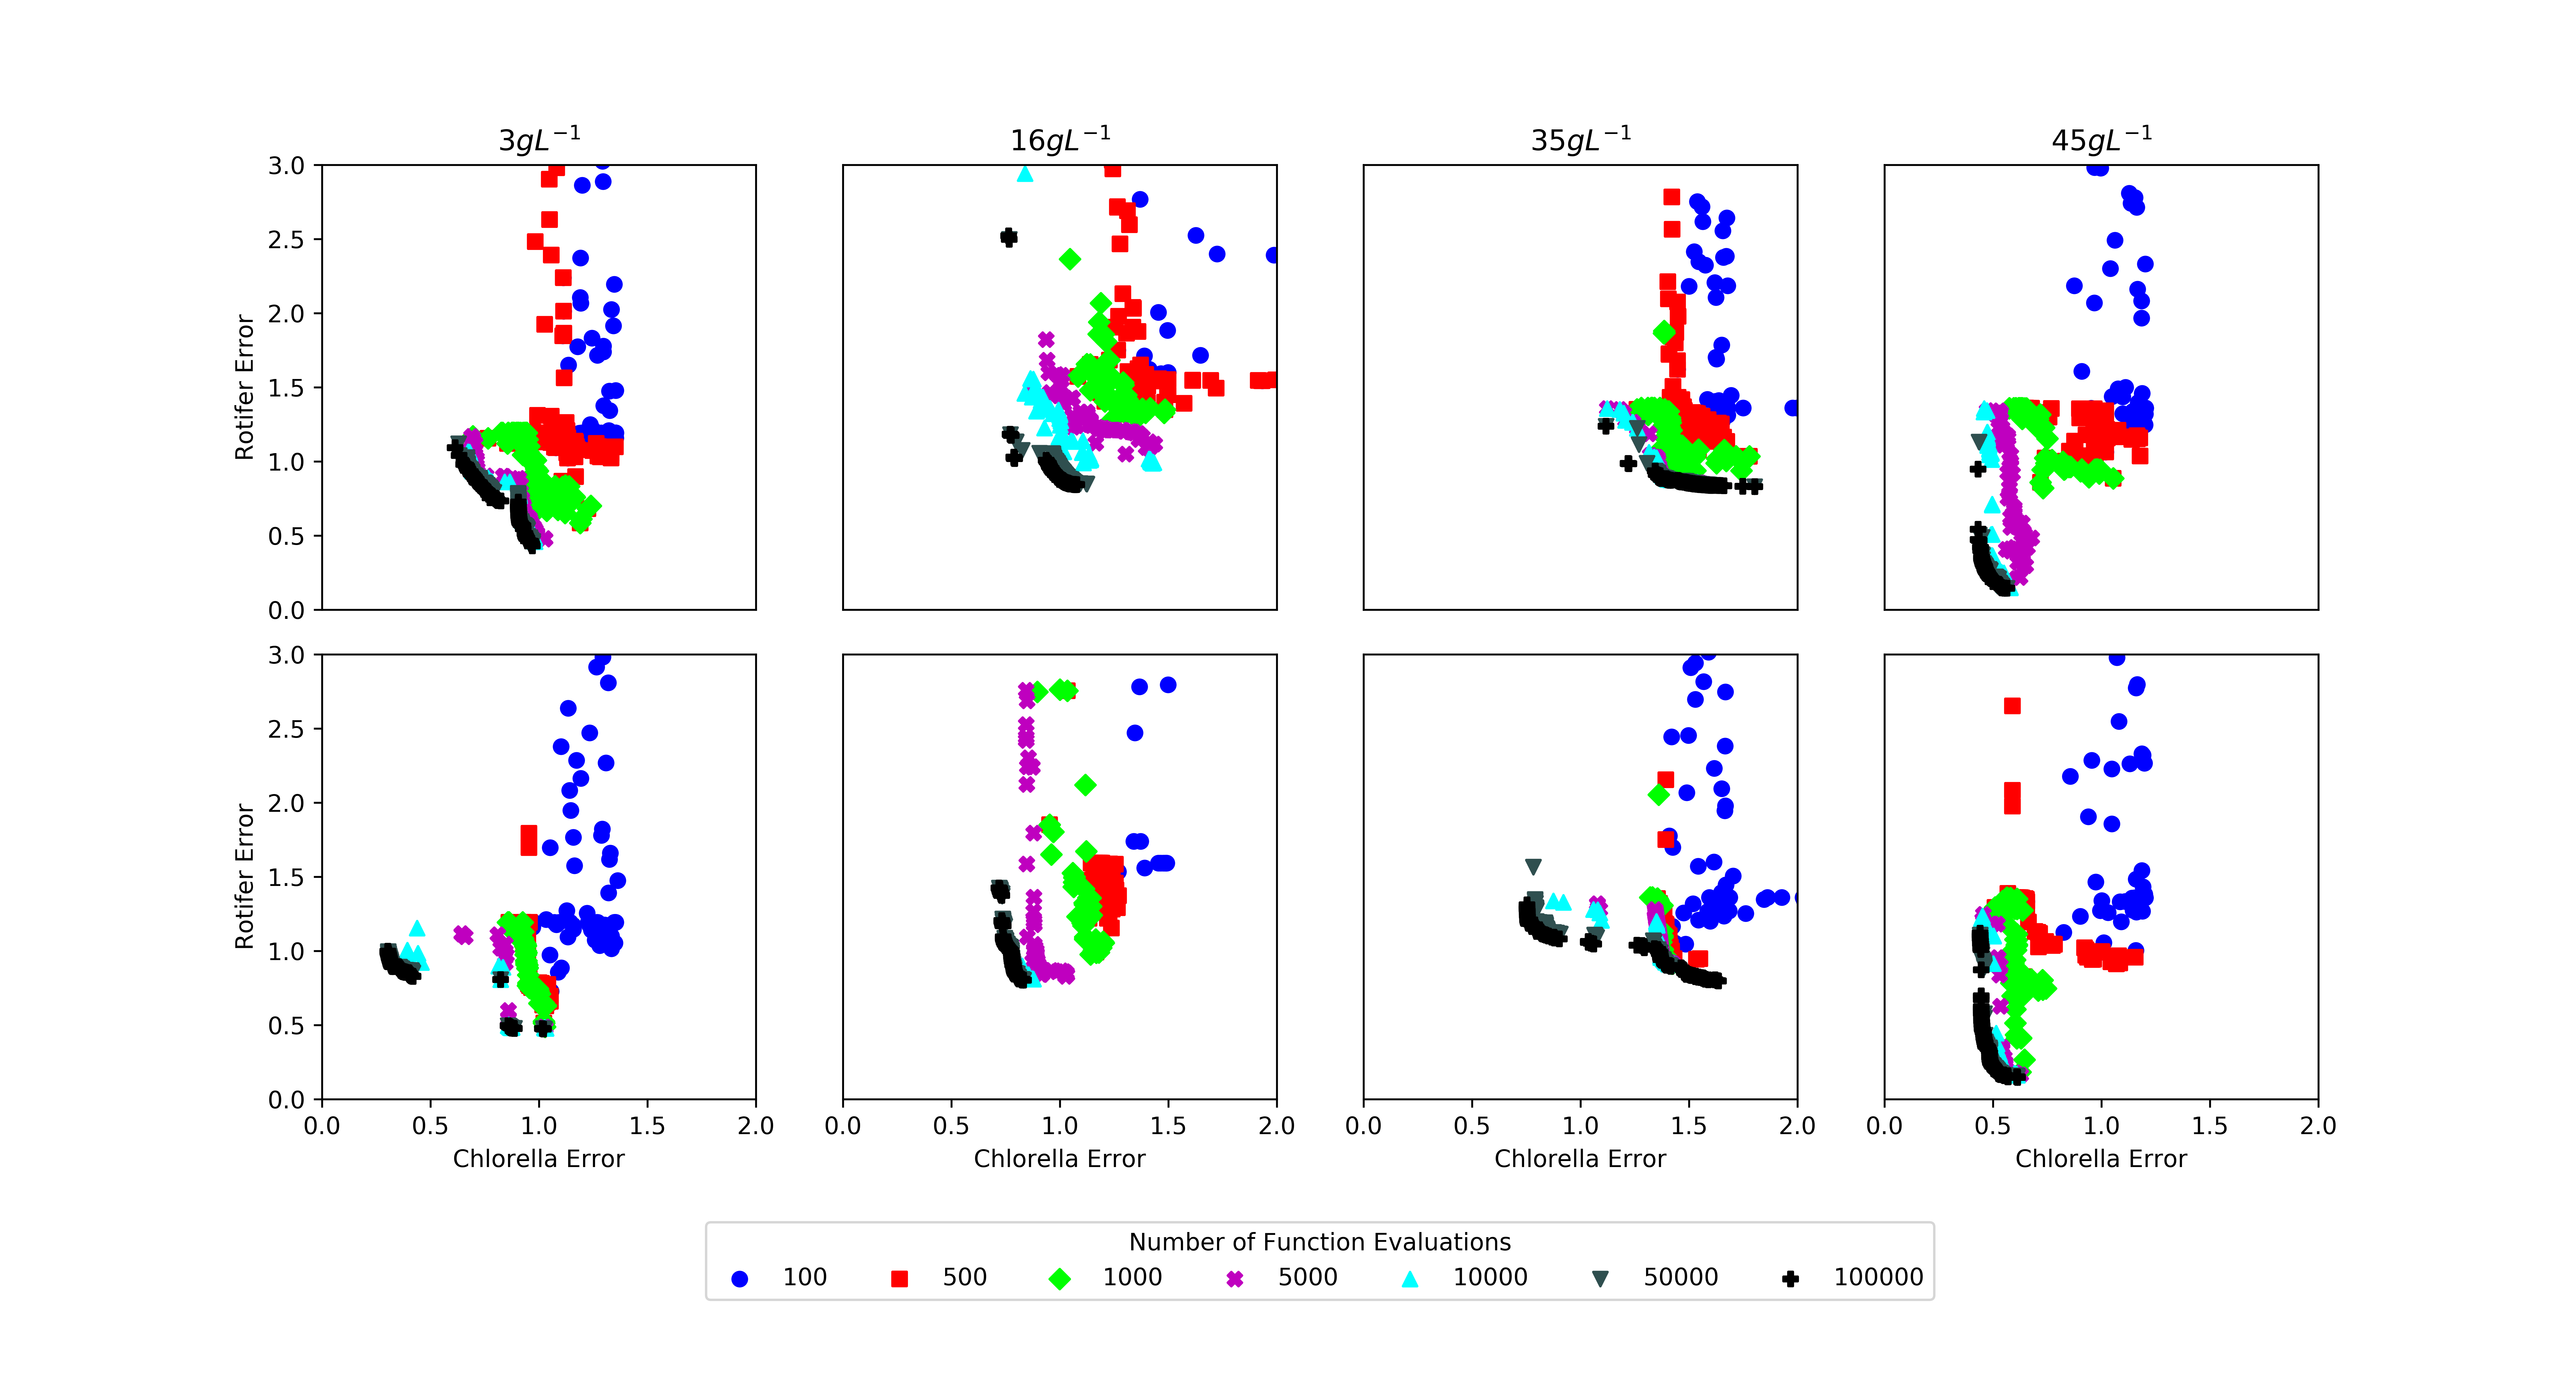
\includegraphics[width=\textwidth]{MOEAConvergence.png}
    \caption{Convergence of the MO algorithms. The first row shows the convergence of NSGAII algorithm and the second row shows the convergence of the SPEA2 algorithm. Each column of figures represents one of the four real data sets. Values for each objective were normalized for readability. Each color represents all solutions after a certain number of function evaluations. As the number of function evaluations increase, the resulting Pareto sets get closer to the ideal point (in this case the origin).}
    \label{fig:MOEAConvergence}
\end{figure}

\indent{} The way that data was generated 

\end{document}

